\section{Konzept}
Ausgehend von unseren Rechercheergebnissen haben wir unseren Fuchsjagd-Sender
folgendermaßen konzipiert.
\subsection{Versorgung}
\begin{figure}[H]
\centering
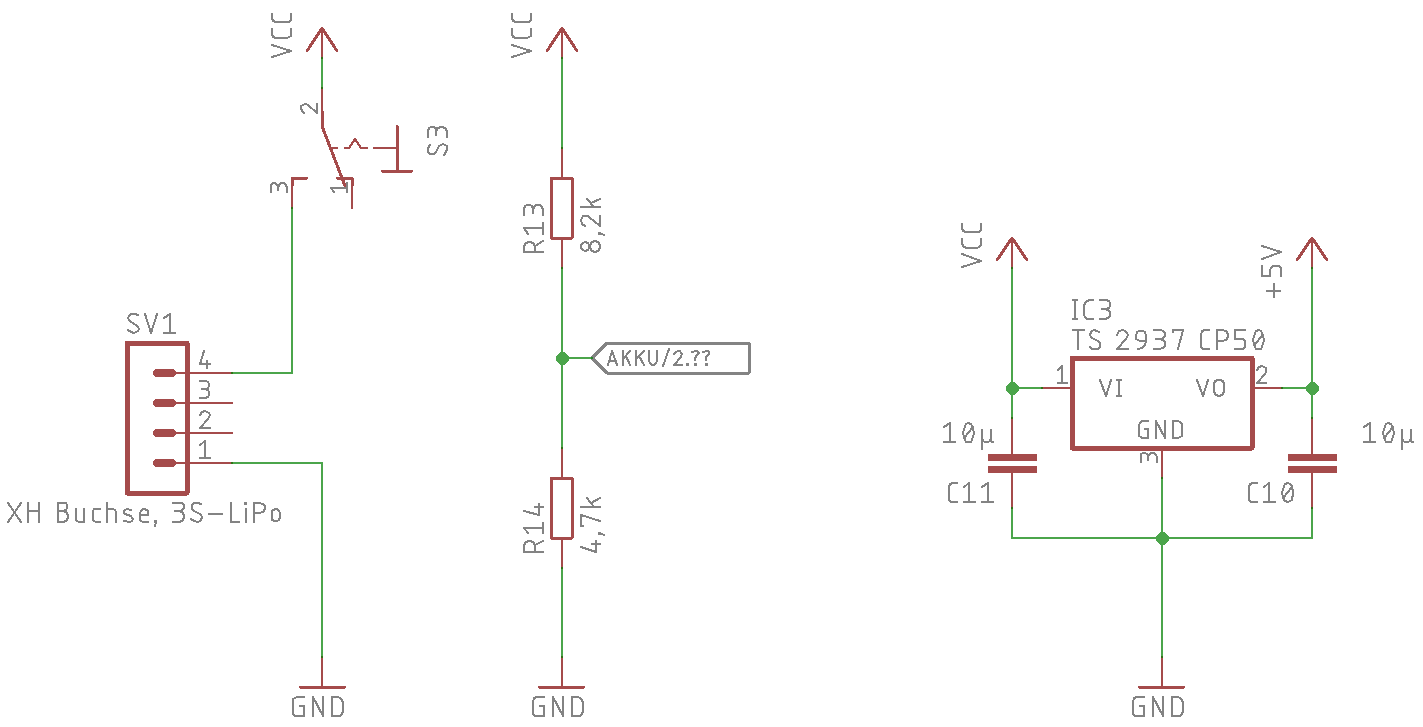
\includegraphics{res/Versorgung.png}
\caption{Versorgung der Platine}
\end{figure}
Die Platine wird über einen dreizelligen Lithium-Polymer-Akku mit einer Nennspannung
von $11,1$V betrieben. Da unter anderem der Mikrocontroller nur mit $5$V versorgt
werden kann, nutzen wir einen Linearregler, der zusätzlich zur Versorgungs-Schiene eine
$5$V Schiene bereitstellt.

\subsection{Der Sender}
Das Sendesignal hat eine Frequenz von $3,5795$MHz und wird direkt vom auf dem Board
verbauten Quarz-Oszillator erzeugt, der zusätzlich dem Mikrocontroller als Takt
dient. Das erzeugte Signal lässt sich von dem Mikrocontroller über ein UND-Gatter steuern. Dieses
Signal wird dann letztendlich von einem FET auf ca. $12$V verstärkt und anschließend gefiltert,
um durch nichtliniearitäten entstandende Oberwellen auszugleichen. Die Verstärkerstufe ist wie folgt aufgebaut:

\begin{figure}[H]
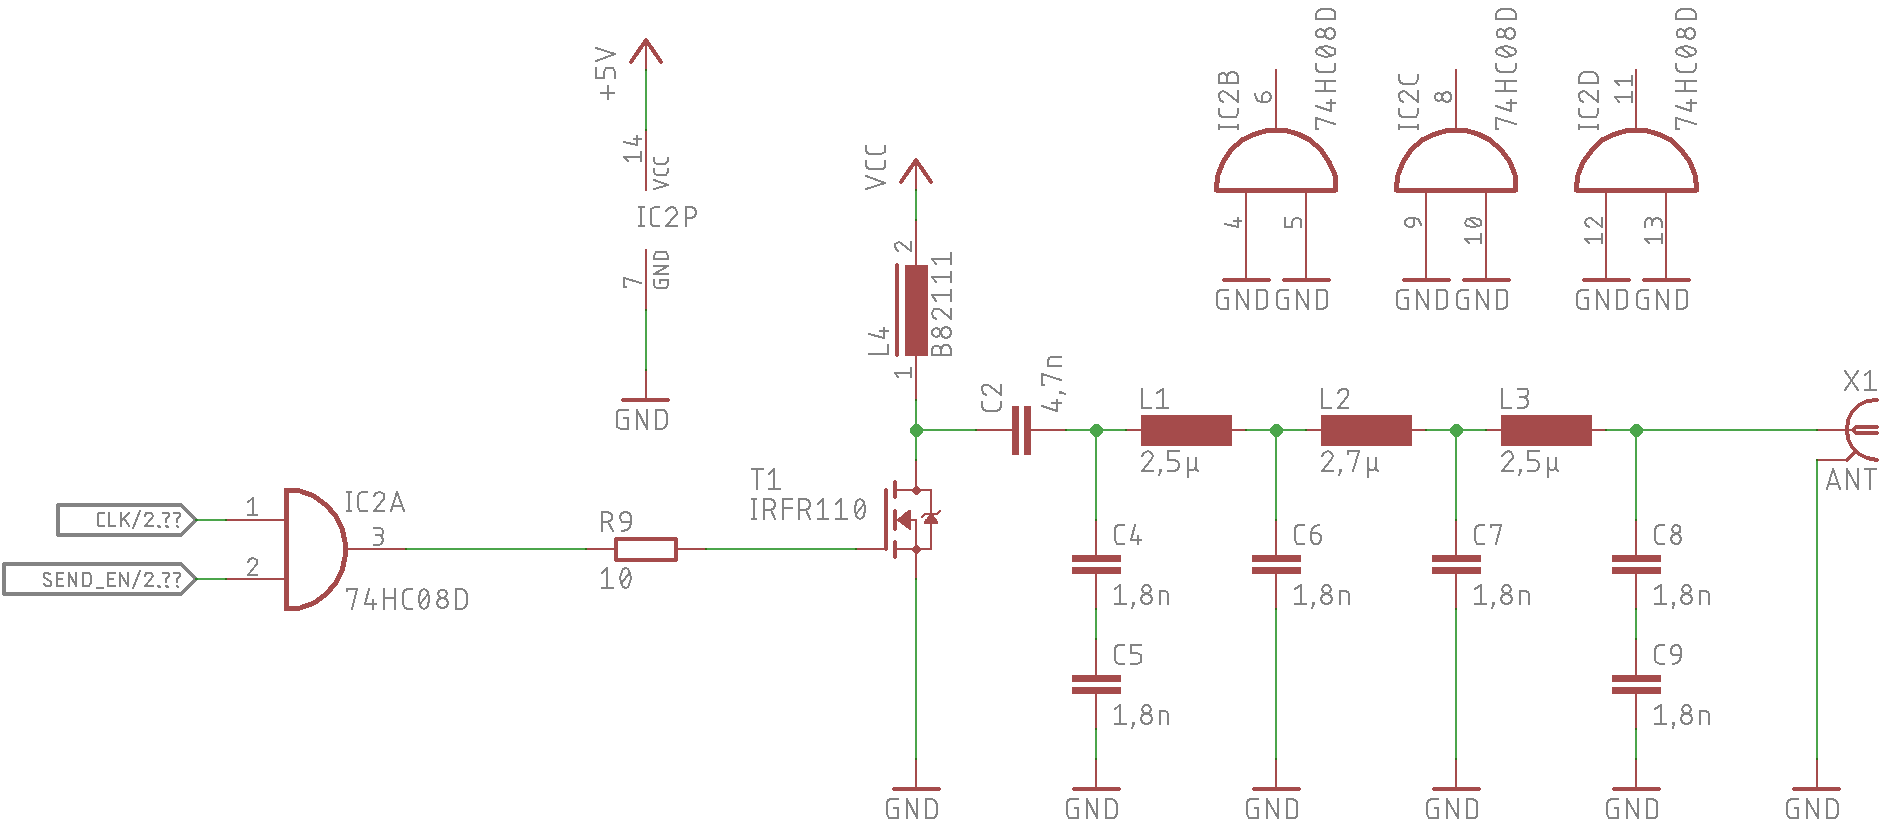
\includegraphics{res/Endstufe.png}
\caption{Verstärkerschaltung des Senders}
\end{figure}

\subsection{Filterung des erzeugten Signals}
Damit der Sender ausschließlich im erlaubten Band sendet, wird der Verstärkerstufe
ein Tiefpassfilter nachgeschaltet. Wir haben uns für einen Tiefpassfilter siebter
Ordnung vom Typ Tschebyscheff entschieden, da es eine sehr hohe Steilheit aufweißt
und die Ripple kein Problem darstellen, da wir ohnehin ein sehr schmalbandiges
Signal senden wollen. Die Kapazitäten wurden zu Werten der E-Reihe modifiziert. Das Filter ist wiefolgt aufgebaut:
\begin{figure}[H]
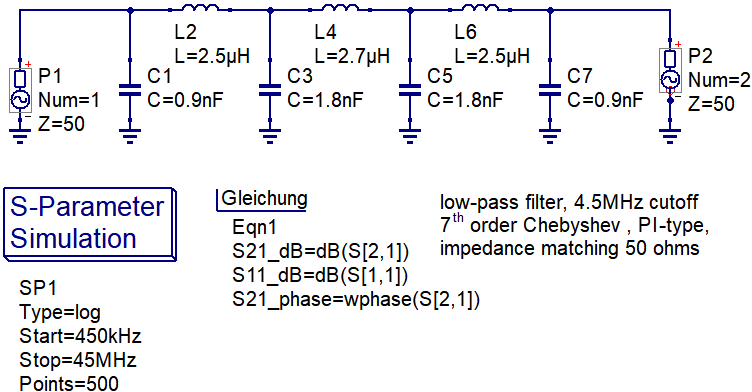
\includegraphics{res/TP_Schaltplan.png}
\caption{Aufbau des Tschebyscheff-Filters}
\end{figure}

\begin{figure}[H]
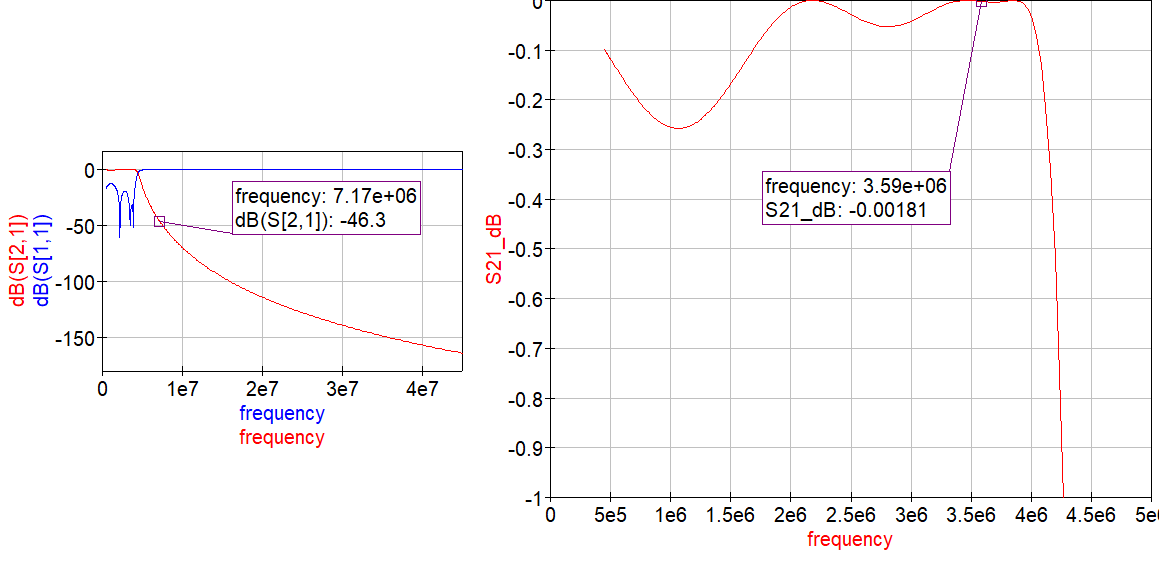
\includegraphics[scale=0.6]{res/TP_Simulation.png}
\caption{Frequenzgang des Filters: Transmission in rot, Reflektionsfaktor in blau}
\end{figure}
Die Simulation zeigt das gewünschte Verhalten des Filters: Bei der gewünschten
Sendefrequenz von $3,5795$MHz beträgt die (ideale) Dämpfung quasi $0$dB.
Die für uns unkritische Welligkeit bleibt unter $0.3$dB.
Die Dämpfung der ersten Oberschwingung beträgt etwa 46dB.

\subsection{Steuerung}
Der Sender wird von einem einfachen Mikrocontroller gesteuert. Dieser muss nur
sehr geringe Anforderungen erfüllen, da er keine aufwendigen Berechnungen oder anderweitige
Aufgaben bewältigen muss. Er muss lediglich in der Lage sein, Daten, wie z.B. das
zu sendende Morsezeichen und die Sendeintervalllänge zu speichern und später dann
den Sender periodisch zu aktivieren. Deshalb haben wir für den Mikrocontroller vom
Typ ATtiny44 entschieden, der alle Voraussetzungen erfüllt. Der Mikrocontroller bekommt
ein externes Clock-Signal vom Quarz-Oszillator, der eine höhere Präzision, als der interne
Oszillator hat. Diese Präzision ist wichtig, da sich sonst auf Dauer die Sendeintervalle von
verschiedenen Sendern überlappen können. Der Mikrocontroller schaltet im Sendebetrieb den Sender
über einen GPIO-Pin und ein UND-Gatter jeweils eine gewisse Zeit ein und aus, je nach eingestelltem
Morsezeichen. Ist das Sendeintervall vorbei, wird der Sender bis zum nächsten Intervall komplett
deaktiviert.

Der Mikrocontroller wird komplett in C programmiert. Dadurch kann die Software flexibler auf die Aufgabe zugeschnitten
werden und es ist daher möglich einen günstigereren Mikrocontroller mit weniger Flash-Speicher zu nutzen.

Der Mikrocontroller ist folgendermaßen beschaltet:

\begin{figure}[H]
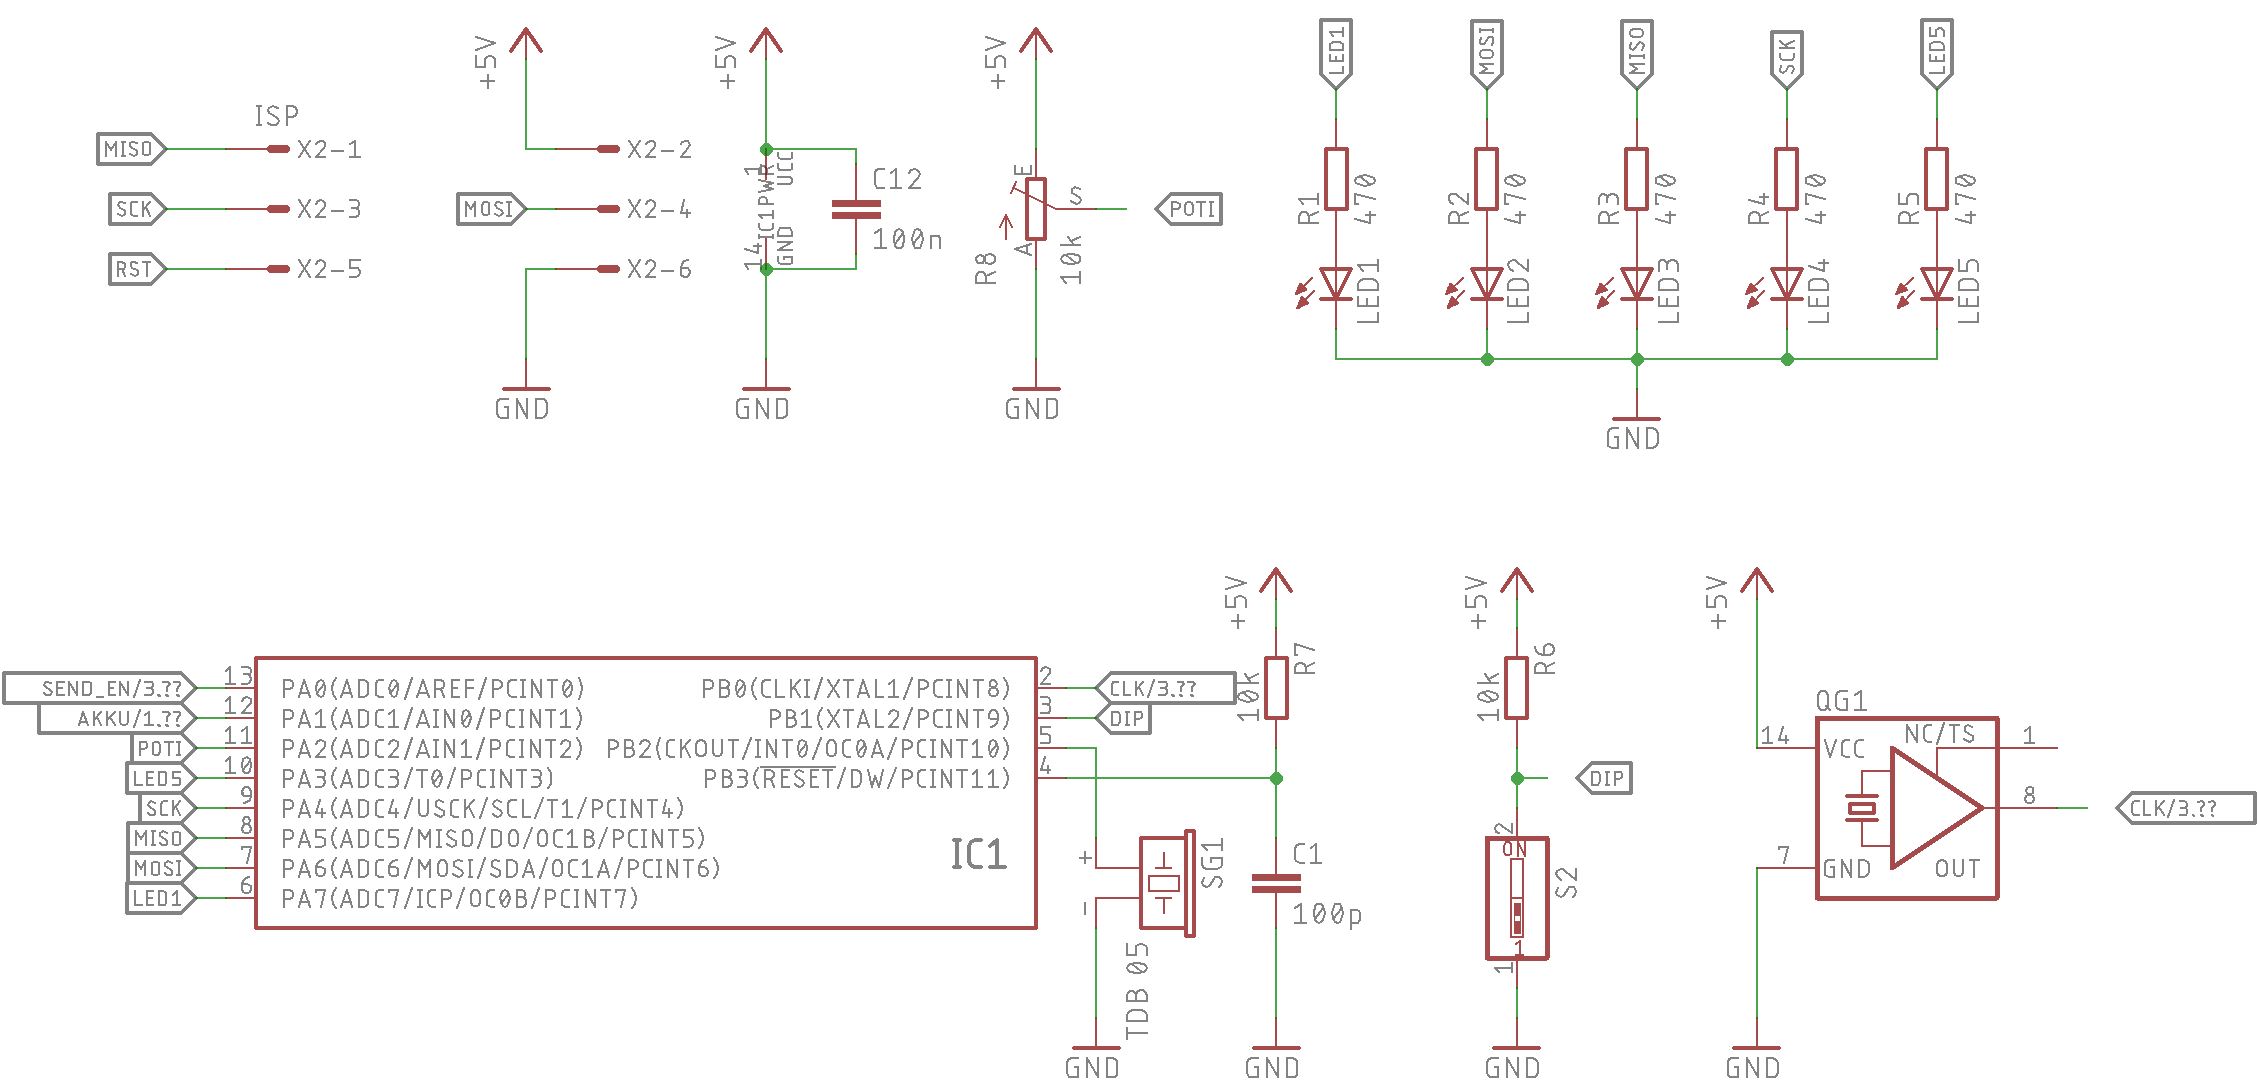
\includegraphics[scale=0.9]{res/Controller.png}
\caption{Beschaltung des Mikrocontrollers}
\end{figure}

\subsection{Bedienung}
Der Fuchsjagd-Sender wird über einen Statusschalter, sowie über ein Potentiometer
gesteuert. Als Anzeige dienen 5 LEDs. Mit dem Statusschalter wird ausgewählt, ob
man das zu sendende Morsezeichen oder die Sendepausen einstellen möchte.
Mit dem Potentiometer wir der eigentliche Wert eingestellt. Über die LEDs wird dieser
Wert in bestimmten Schritten angezeigt. Einmal eingestellt, sendet der Sender das gewünschte
Morsezeichen in den festgelegten Zeitabständen für jeweils eine feste Zeitdauer. Für die Bedienung ist ein passender Schraubenzieher erforderlich.\\
Bei der aktuellen Programmierung des Mikrocontrollers sind die möglichen Intervalle 10, 20, 30, 45, 60, 120, 240 und 600 Sekunden.
Die möglichen Sendesymbole sind A, E, I, O, U, T, M, N. \\
Der Code ist dabei so geschrieben, dass die möglichen Intervalllängen und Symbole, sowie die Schrittweite einfach, also durch Ändern eines einzelnen Wertes, auszutauschen sind.
